\section{Conclusion}

\pgfdeclareimage[width=1.0\paperwidth]{header-image}{header_images/post_fire}

\begin{frame}<1-4>
    \frametitle{Humans reduce burnt area}
	\begin{itemize}
		\large{
			\item Ignitions generally do not limit burnt area
			\item Suppression efforts and land use have much bigger impact
		}
	\end{itemize}
	\visible<2->{
		\huge{BUT...}
		\begin{itemize}
			\large{
				\item Human fires are a significant ignition source, particularly in pasture areas
				\item And would likely effect other aspects of fire regime (fire size, intensity etc)
			}
		\end{itemize}
	}
\end{frame}

\addtocounter{framenumber}{-1}
\begin{frame}
	\frametitle{Tipping points and model assessment}
	\framesubtitle{}
	
	\begin{textblock*}{12cm}(0cm,1.5cm)
		\begin{tikzpicture}
		\node[anchor=south west,inner sep=0] (image) at (0,0) {
			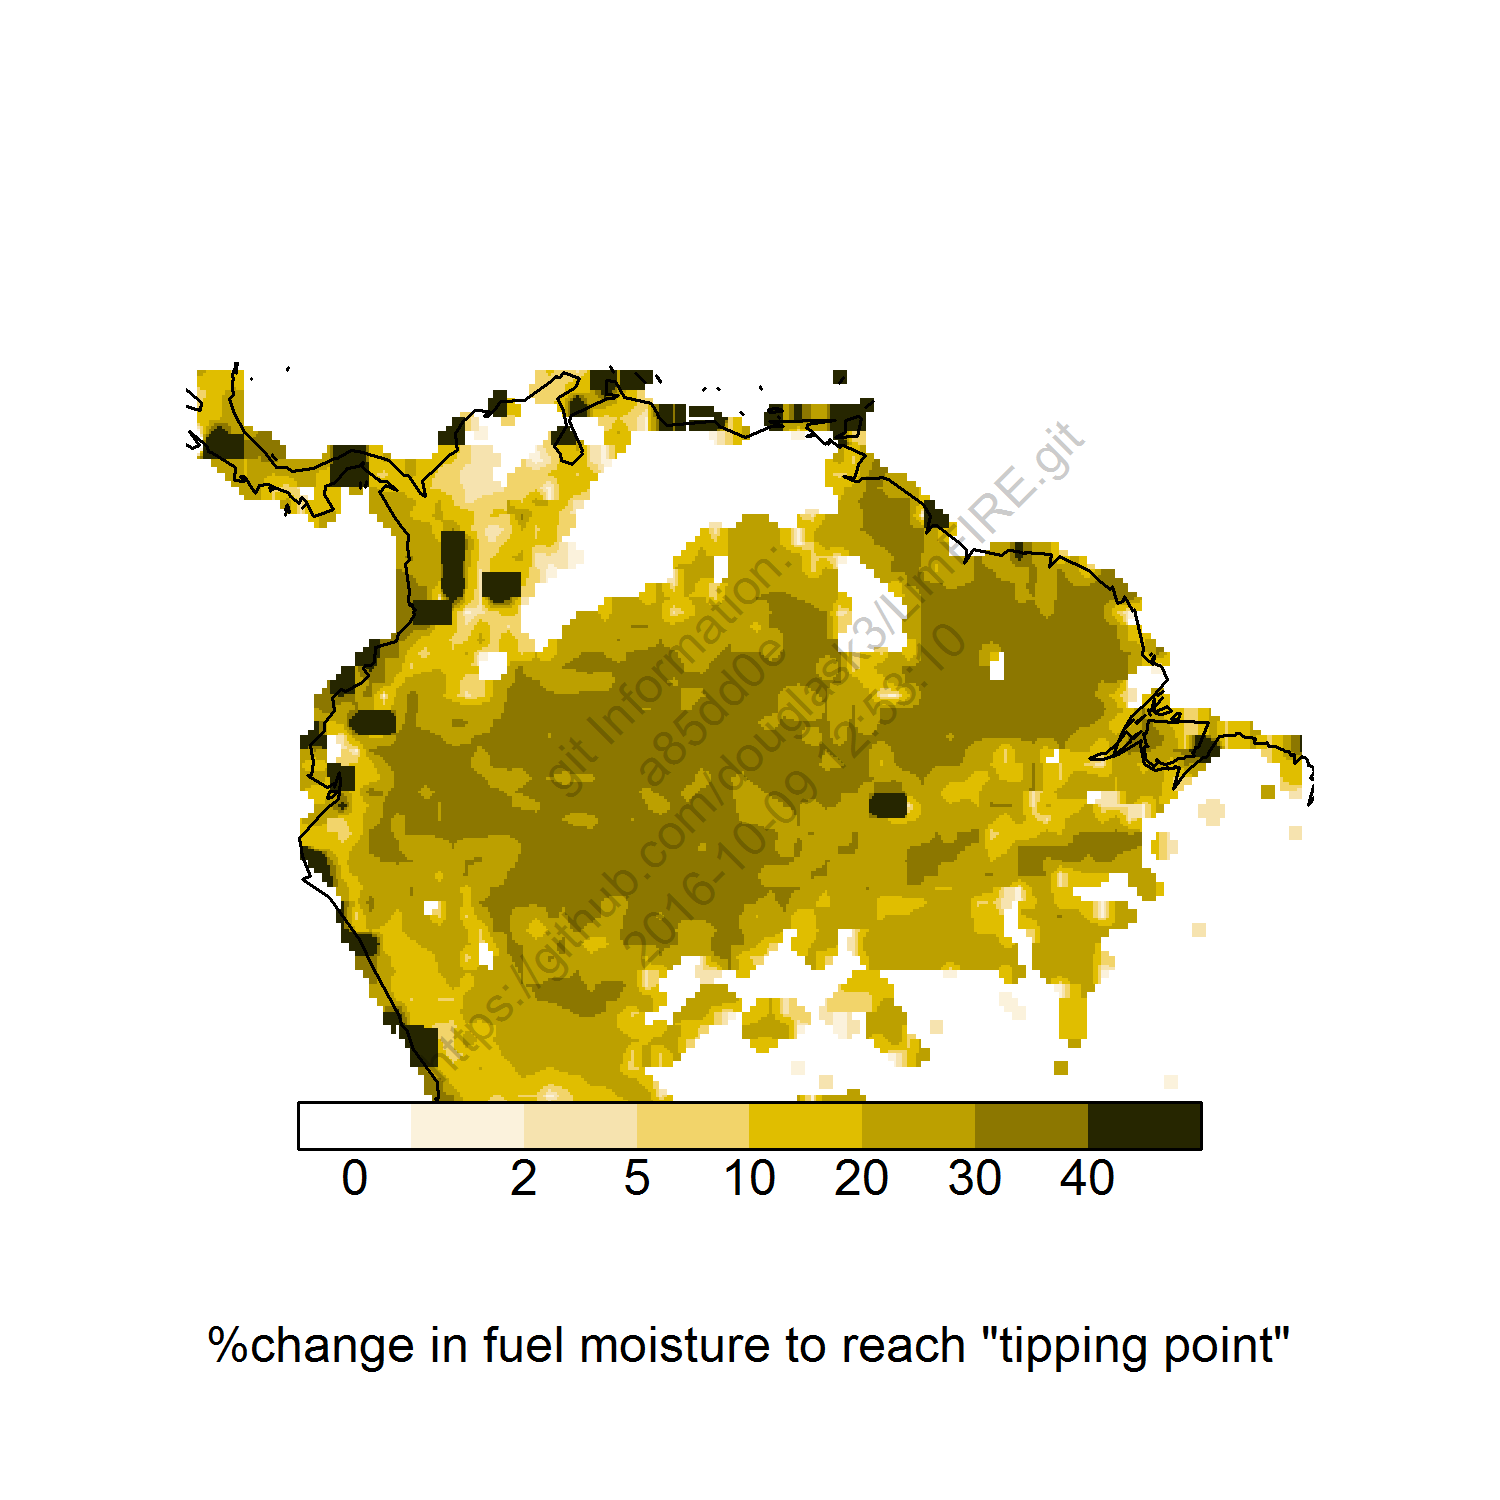
\includegraphics[width=4.5cm]{images/tippingPoint}
		};
		\end{tikzpicture}
	\end{textblock*}
	\begin{textblock*}{12cm}(5cm,1.5cm)
		\begin{tikzpicture}
		\node[anchor=south west,inner sep=0] (image) at (0,0) {
			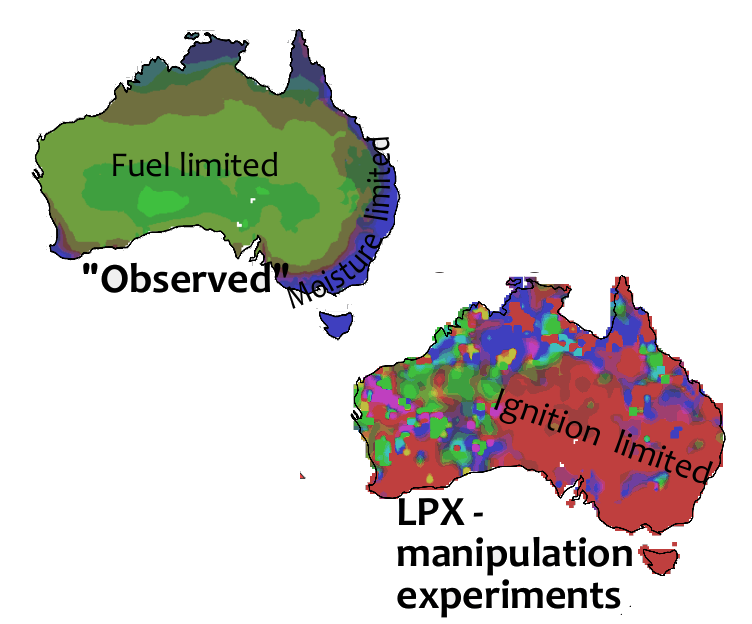
\includegraphics[width=5.0cm]{images/ModComp}
		};
		\end{tikzpicture}
	\end{textblock*}
\end{frame}

\addtocounter{framenumber}{-1}
\begin{frame}
	\frametitle{Ignitions}
	\framesubtitle{Which is more important}
	
	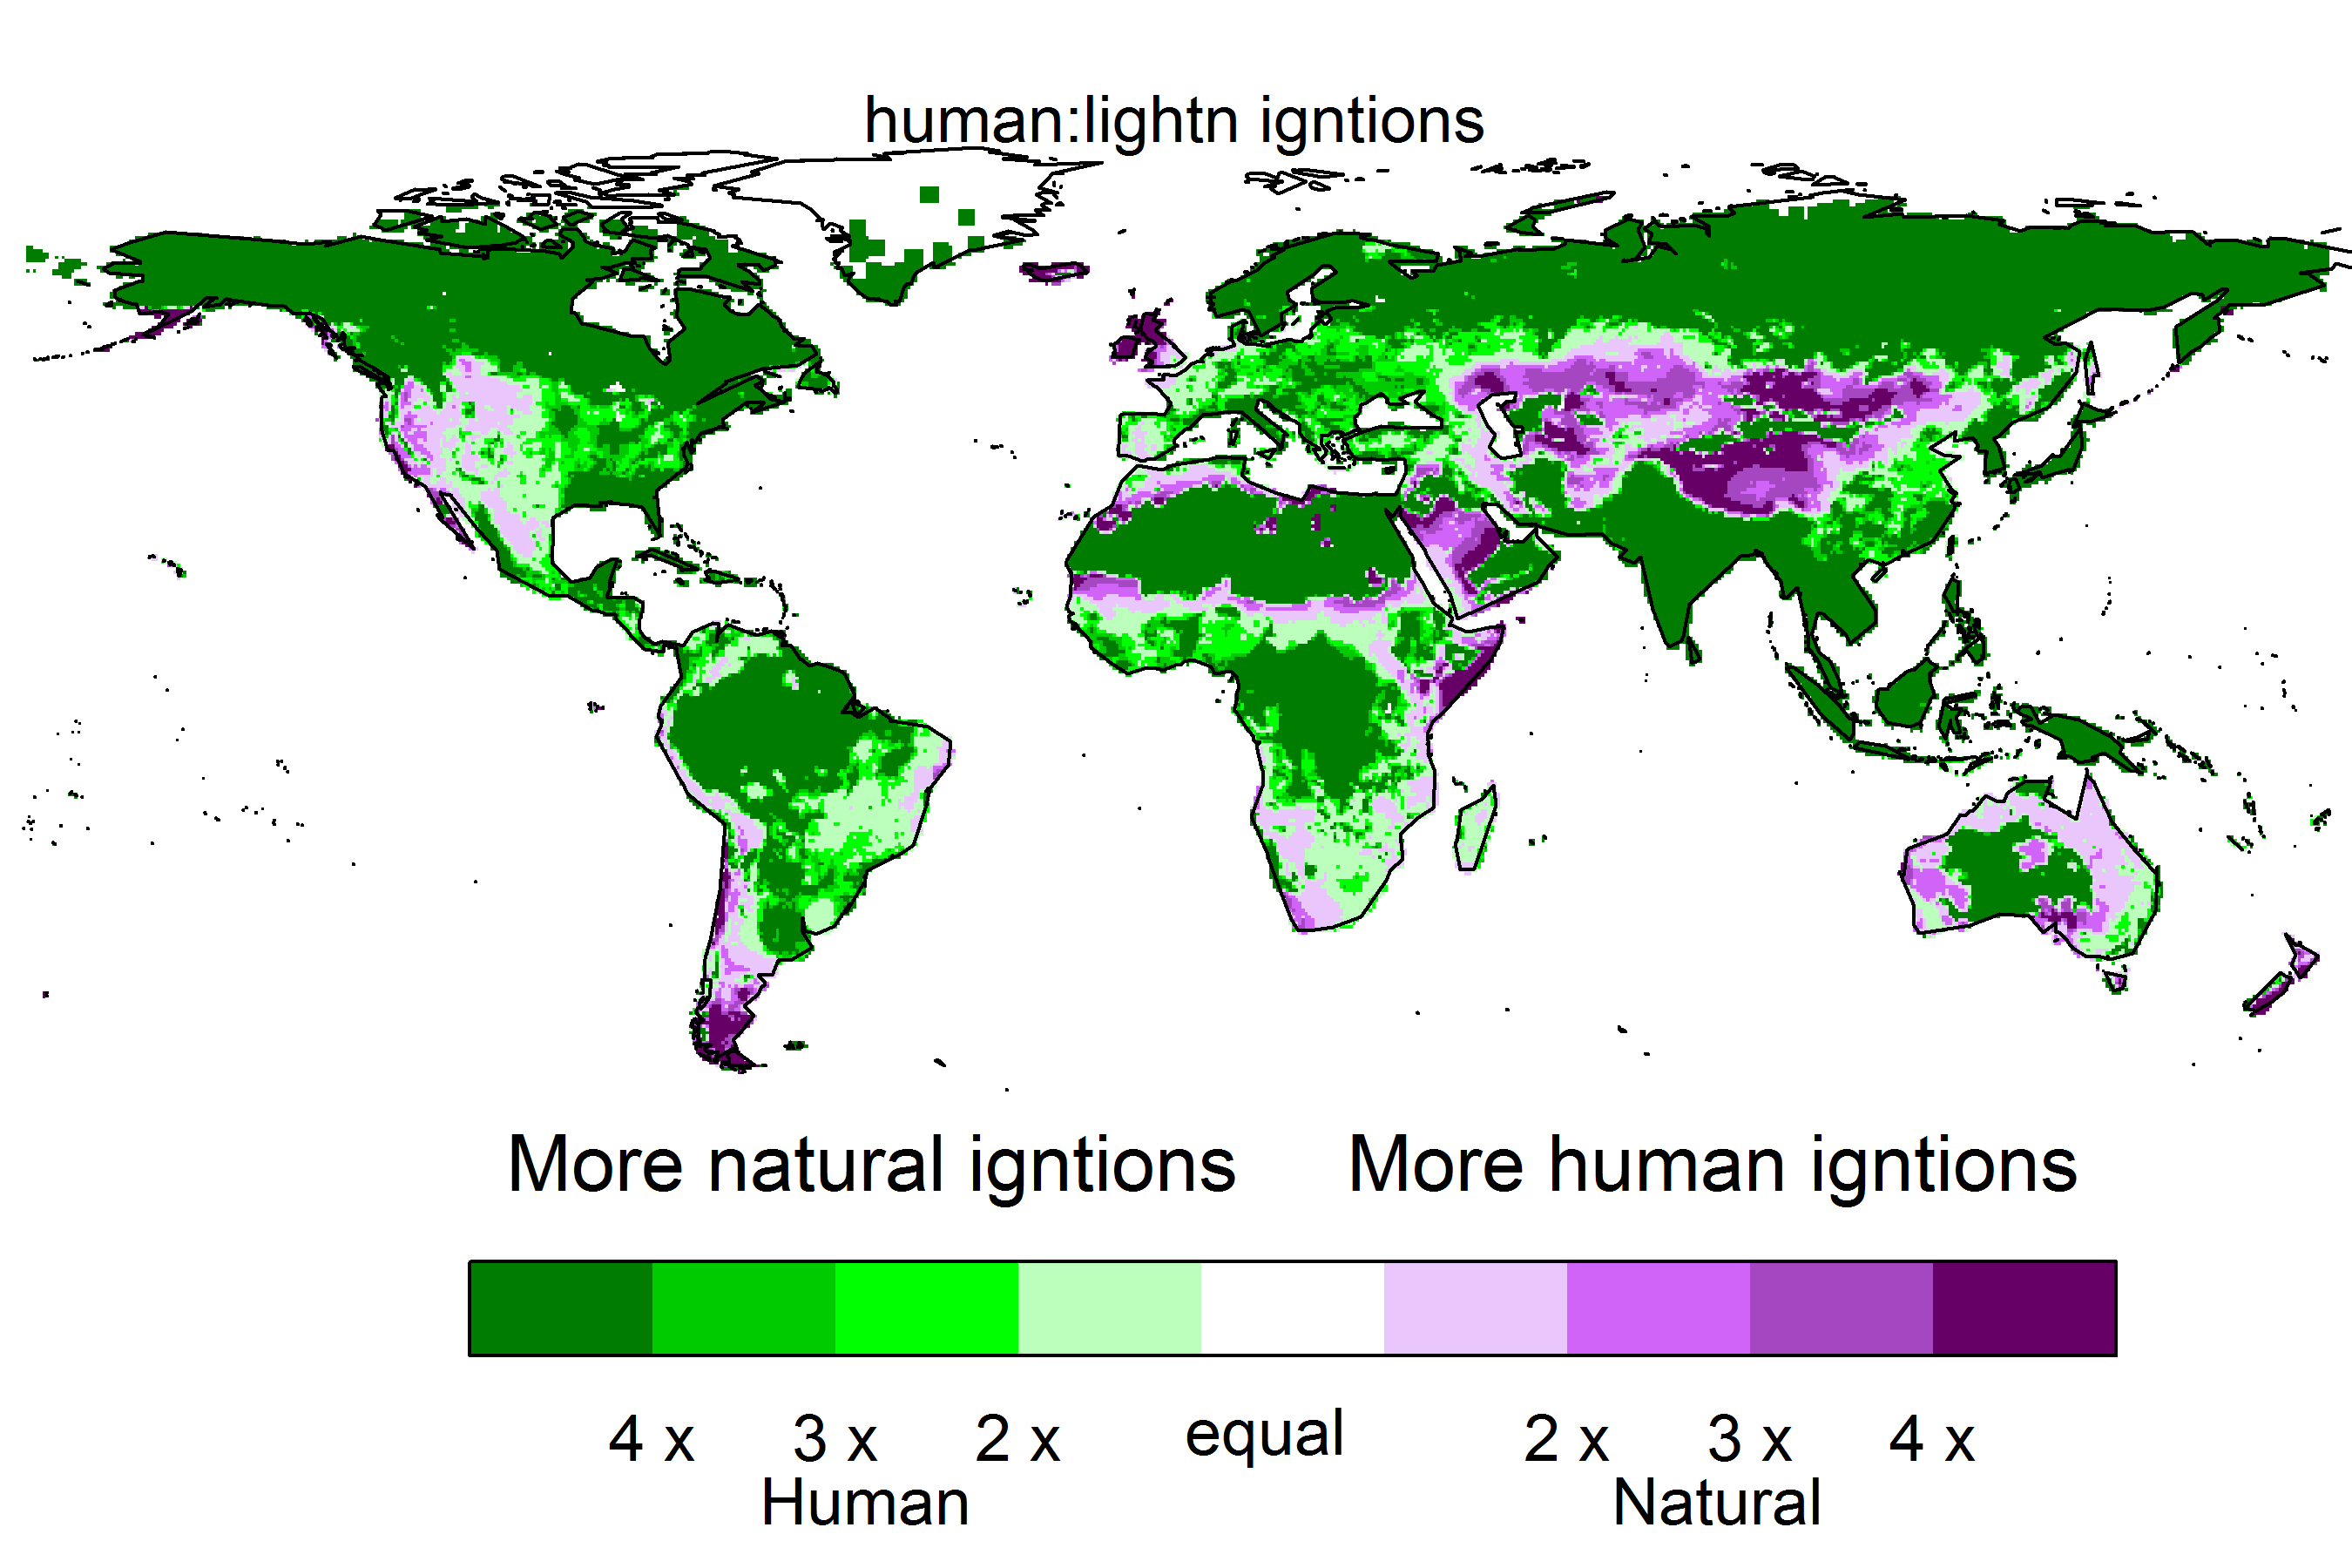
\includegraphics[width=11.0cm]{images/igntitions/IgntionInfosourceImportance}
\end{frame}


%\begin{frame}
%    \frametitle{Acknowledgments}
%    \framesubtitle{Questions..?}
%\end{frame}
\addtocounter{framenumber}{-1}
\begin{frame}<5>
    \frametitle{Sensitivity to Controls}
    \controlsSide{limitation_map}
\end{frame}
